\documentclass{article}
\usepackage{tikz}
\usetikzlibrary{arrows.meta}

\begin{document}

\begin{center}
    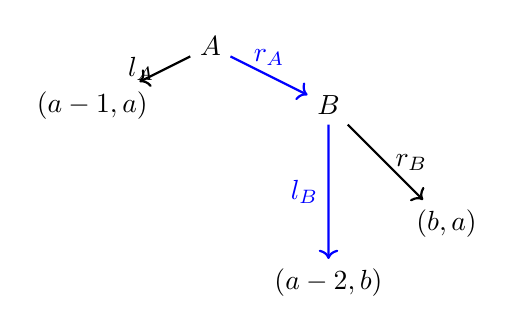
\begin{tikzpicture}[scale=1.5]
        % Nodes
        \node (A) at (0, 0) {$A$};
        \node (B) at (1, -0.5) {$B$};
        \node (C) at (-1, -0.5) {$(a-1,a)$};
        \node (D) at (2, -1.5) {$(b,a)$};
        \node (E) at (1, -2) {$(a-2,b)$};

        % Edges
        \draw[->, thick] (A) -- node[left] {$l_A$} (C);
        \draw[->, thick, blue] (A) -- node[above] {$r_A$} (B);
        \draw[->, thick, blue] (B) -- node[left] {$l_B$} (E);
        \draw[->, thick] (B) -- node[right] {$r_B$} (D);
    \end{tikzpicture}
\end{center}

Game \( G \) with \( a > 0 \), honest history \(\color{blue}{(r_A, l_B)}\).

\end{document}